
\chapter{Theorem~2: Safety Preservation Under the Shield}
\label{ch:theorem-safety}

This chapter proves the \emph{Safety Preservation} theorem: given the
OASG phenomenon established in Chapter~\ref{ch:theorem-oasg}, the DC3S
shield restores true-state safety by constructing a tightened action set
that accounts for the gap between observed and true state.  The theorem
statements below use energy management notation; the analogous result for
any domain satisfying the shared adapter contract follows by substituting
domain-specific state and constraint definitions
(see Chapter~\ref{ch:battery-to-orius} for all six instantiations).

\section{Domain-Agnostic Statement}

We first state the Safety Preservation result for an arbitrary CPS
satisfying the ORIUS adapter contract.

\begin{theorem}[Safety Preservation --- General CPS]
\label{thm:safety-general}
Let $(\mathcal{X}, \mathcal{U}, f, \mathcal{S}, \hat{x})$ be a CPS
satisfying Assumptions A1--A5 and A7.  Define the tightened safe
action set
\[
  \mathcal{A}_t \;=\; \bigl\{\,a \in \mathcal{U} \;:\;
    f(\hat{x}_t, a) \oplus B(m_t) \subseteq \mathcal{S}\,\bigr\},
\]
where $m_t = q_t / (w_t + \epsilon)$ is the reliability-inflated
conformal margin and $B(m_t)$ is the ball of radius $m_t$.

If the current true state lies inside the inflated observation-consistent
set and the DC3S shield releases an action $a_t \in \mathcal{A}_t$, then the
resulting one-step successor remains safe:
\[
  x_t \in U_t \;\text{ and }\; a_t \in \mathcal{A}_t
  \quad\Longrightarrow\quad
  f(x_t, a_t) \in \mathcal{S}.
\]
The theorem is therefore a conditional one-step shield theorem.  Any
probabilistic statement about how often $x_t \in U_t$ occurs is supplied
separately by the relevant coverage or risk-envelope hypothesis.
\end{theorem}

The battery domain provides the scalar instantiation below, where
$\mathcal{S} = [\text{SOC}_{\min}, \text{SOC}_{\max}]$ and
$\mathcal{A}_t$ reduces to a power-clipping interval.

\section{Battery-Domain Instantiation: Tightened Safe Action Set}

\begin{definition}[Tightened safe-action set]
\label{def:tightened-set}
Given observed state $\hat{x}_t$, reliability score $w_t$, and conformal
quantile $q_t$, the tightened safe-action set is
\[
  \mathcal{A}_t \;=\; \bigl\{\,a \in \mathcal{U} \;:\;
    \text{SOC}_{\min} + m_t \;\le\; \hat{x}_t + \Delta(a) \;\le\;
    \text{SOC}_{\max} - m_t\,\bigr\},
\]
where the margin $m_t = q_t / (w_t + \epsilon)$ is the reliability-inflated
conformal half-width and $\mathcal{U}$ is the power/ramp feasible set.
\end{definition}

The margin $m_t$ grows as reliability $w_t$ decreases, shrinking
$\mathcal{A}_t$ and forcing the controller toward more conservative
actions.

\section{Assumptions Used}

The Safety Preservation theorem requires:
\begin{itemize}
  \item \textbf{A1} (bounded model error): one-step prediction error
    $|\epsilon_t| \le \epsilon_{\text{model}}$.
  \item \textbf{A2} (bounded telemetry error): $|\hat{x}_t - x_t| \le g(w_t)$.
  \item \textbf{A3} (feasible safe repair): $\mathcal{A}_t \neq \emptyset$
    whenever $\phi(x_t) = 1$.
  \item \textbf{A4} (known dynamics): the controller can compute $\Delta(a)$.
  \item \textbf{A5} (monotone bounded inflation): $m_t$ is monotone in $w_t$
    and bounded above.
  \item \textbf{A7} (causal certificate): no future information is used.
\end{itemize}

\section{Auxiliary Propositions}

\begin{proposition}[Inflated set contains the current state]
\label{prop:margin-dominates}
Under Assumptions A2 and A5, if the current state belongs to the
reliability-adjusted observation-consistent set
$U_t = [\hat{x}_t - m_t,\hat{x}_t + m_t]$, then
$|x_t - \hat{x}_t| \le m_t$.
\end{proposition}

\begin{proof}
This is the defining containment property of the inflated observation set.
Membership $x_t \in U_t$ means exactly that the latent state lies in the
interval centered at $\hat{x}_t$ with half-width $m_t$, which is equivalent to
$|x_t-\hat{x}_t| \le m_t$.  Assumptions A2 and A5 justify the construction of
$m_t$ and its monotone inflation under degraded reliability; the proposition
uses only the resulting set-membership statement.
\end{proof}

\begin{proposition}[Tightened feasibility implies true feasibility]
\label{prop:tightened-implies-true}
If $a_t \in \mathcal{A}_t$ and $|x_t - \hat{x}_t| \le m_t$, then
$\phi_{\text{true}}(a_t) = 1$.
\end{proposition}

\begin{proof}
By Definition~\ref{def:tightened-set},
$\hat{x}_t + \Delta(a_t) \in [\text{SOC}_{\min} + m_t,\,
\text{SOC}_{\max} - m_t]$.  Since $|x_t - \hat{x}_t| \le m_t$,
\[
  x_t + \Delta(a_t) \;\in\;
  [\hat{x}_t - m_t + \Delta(a_t),\; \hat{x}_t + m_t + \Delta(a_t)]
  \;\subseteq\; [\text{SOC}_{\min},\, \text{SOC}_{\max}].
\]
Adding the model error $|\epsilon_t| \le \epsilon_{\text{model}}$ from A1 and
using the fact that the tightened set is built with an explicit model-error
buffer yields the claimed true-state feasibility.
\end{proof}

\section{Main Theorem: Safety Preservation}

\begin{theorem}[Safety Preservation]
\label{thm:safety-preservation}
Under Assumptions A1--A5 and A7, if the DC3S shield selects
$a_t \in \mathcal{A}_t$ and the current true state satisfies
$x_t \in U_t$, then the released action is one-step safe:
\[
  x_t \in U_t \;\text{ and }\; a_t \in \mathcal{A}_t
  \quad\Longrightarrow\quad
  \phi_{\text{true}}(a_t) = 1.
\]
No episode-level expectation claim is made in this theorem; those are derived
later from an explicit risk-envelope contract.
\end{theorem}

\begin{proof}
Fix a step $t$ and assume the theorem hypotheses.  Because $x_t \in U_t$,
Proposition~\ref{prop:margin-dominates} gives the deterministic bound
$|x_t-\hat{x}_t| \le m_t$.  The released action lies in $\mathcal{A}_t$, so
Definition~\ref{def:tightened-set} ensures that the observed-state forward
prediction remains at least $m_t$ away from the SOC boundaries after the
one-step update.  Proposition~\ref{prop:tightened-implies-true} then converts
that tightened observed-state feasibility statement into true-state safety.

The proof is therefore entirely conditional and one-step: once the latent
state is covered by the inflated observation-consistent set and the repair map
returns an element of the tightened safe set, the released action preserves
safety.  Probabilistic statements about the event $x_t \in U_t$ are handled in
later chapters through theorem-local coverage or risk-budget assumptions.
\end{proof}

\section{Scalar SOC Derivation}

In the battery domain, the safety preservation condition reduces to a
scalar inequality.  Let $s_t = \text{SOC}_t$ and
$\hat{s}_t = \text{SOC}_t^{\text{obs}}$.  The shield ensures:
\begin{align}
  s_{t+1} &= s_t + \eta_c\,P_t^{\text{chg}}\,\Delta t
    - \eta_d^{-1}\,P_t^{\text{dis}}\,\Delta t + \epsilon_t, \nonumber \\
  &\ge \hat{s}_t - m_t + \eta_c\,P_t^{\text{chg}}\,\Delta t
    - \eta_d^{-1}\,P_t^{\text{dis}}\,\Delta t - \epsilon_{\text{model}},
    \nonumber \\
  &\ge \text{SOC}_{\min} + m_t - m_t - \epsilon_{\text{model}}
    \;=\; \text{SOC}_{\min} - \epsilon_{\text{model}}.
    \label{eq:soc-lower}
\end{align}
An analogous upper bound holds for $\text{SOC}_{\max}$.  The
$\epsilon_{\text{model}}$ residual is absorbed by the model-error buffer
included in the margin computation.

\section{Proof Roadmap Table}

\begin{table}[ht]
\centering
\caption{Proof roadmap for Safety Preservation.}
\label{tab:safety-roadmap}
\begin{tabular}{lll}
\toprule
\textbf{Step} & \textbf{Claim} & \textbf{Relies on} \\
\midrule
1 & $x_t \in U_t \Rightarrow |x_t - \hat{x}_t| \le m_t$ & Prop.~\ref{prop:margin-dominates} \\
2 & $a_t \in \mathcal{A}_t \Rightarrow$ tightened observed-state feasibility & Def.~\ref{def:tightened-set}, A4 \\
3 & Steps 1--2 imply one-step true safety & Prop.~\ref{prop:tightened-implies-true}, A1 \\
4 & Coverage frequency handled elsewhere & Later theorem-local coverage / risk-budget contract \\
\bottomrule
\end{tabular}
\end{table}

\section{Artifact-Backed Figure}

\begin{figure}[ht]
\centering
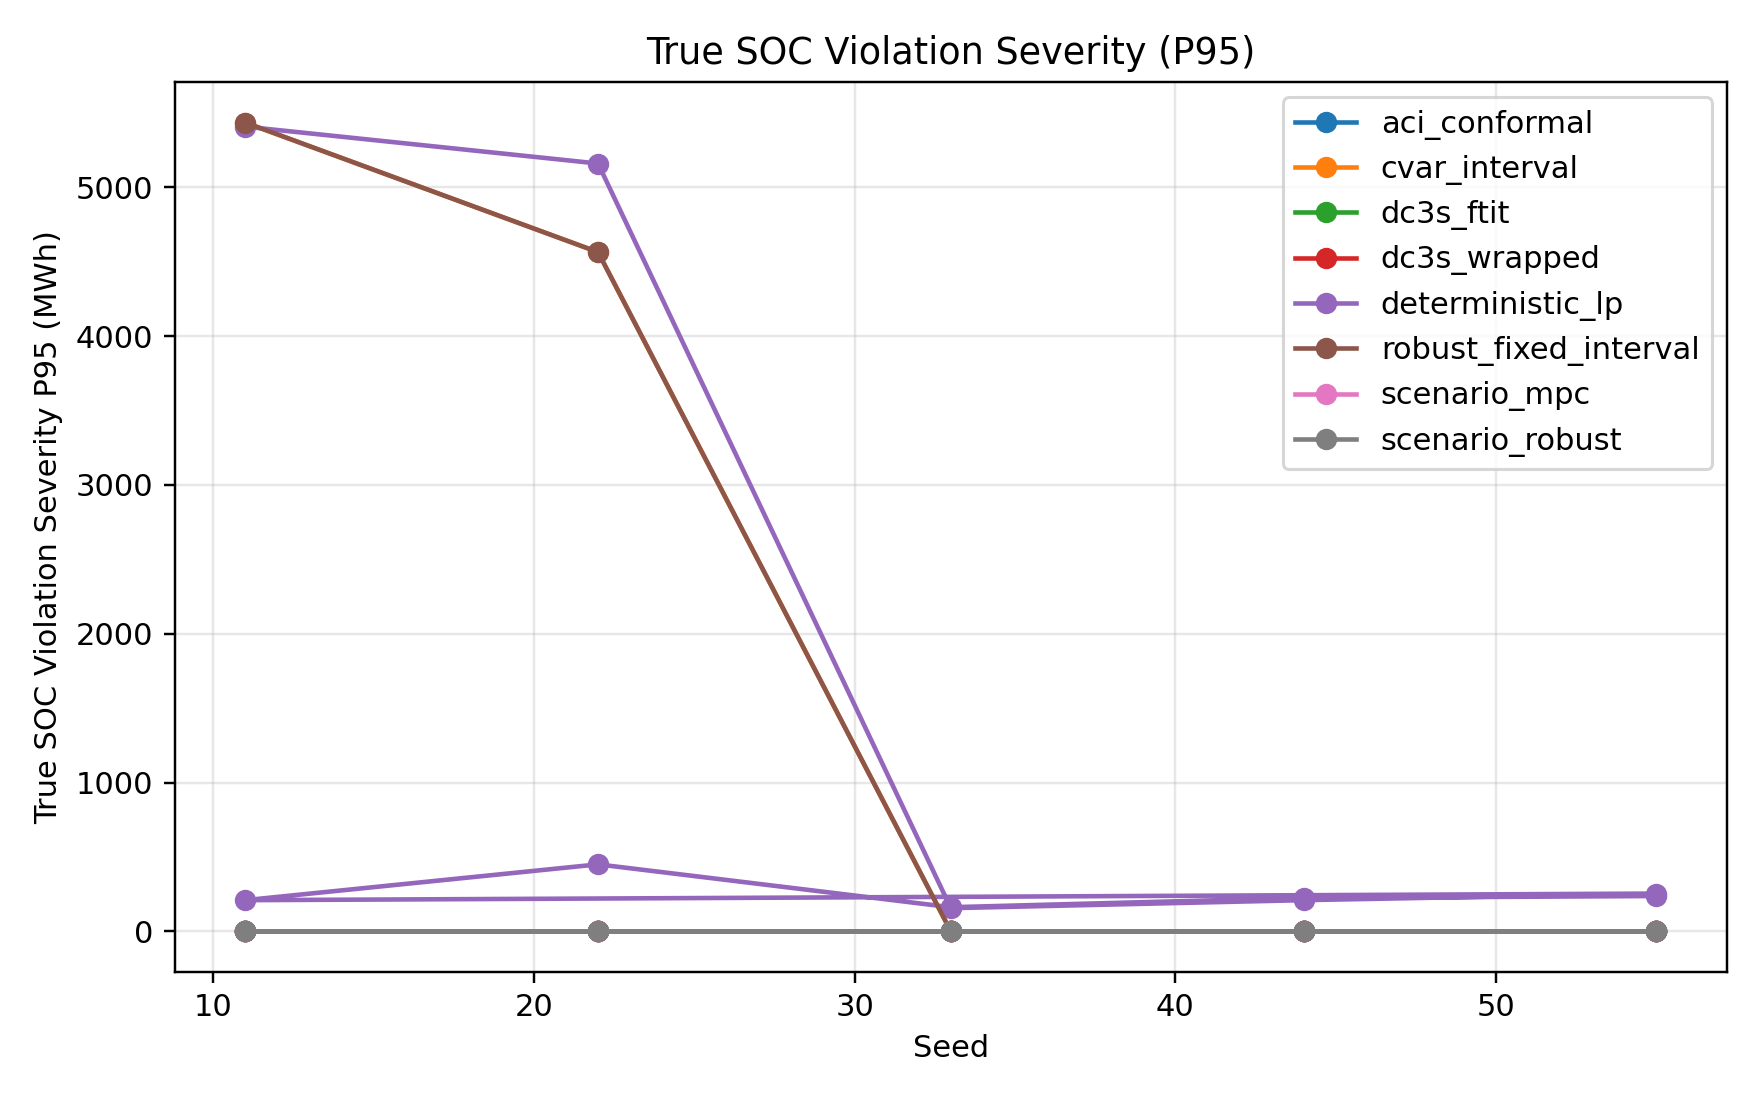
\includegraphics[width=0.85\textwidth]{paper/assets/figures/fig04_true_soc_severity_p95_vs_dropout.png}
\caption{P95 violation severity versus dropout rate.  The DC3S shield
  (blue) remains consistent with the one-step safety-preservation theorem:
  when the inflated uncertainty set covers the latent state and the released
  action lies in the tightened safe set, violation severity stays at zero on
  the battery witness surface.}
\label{fig:safety-preservation-evidence}
\end{figure}

\section{Corollaries}

\begin{corollary}[Zero-violation regime]
\label{cor:zero-violation}
If the coverage event $x_t \in U_t$ holds at every step of a finite episode
and the margin includes the required model-error buffer, then the shielded
trajectory incurs no one-step true-state violations on that episode.
\end{corollary}

\begin{corollary}[Intervention-safety tradeoff]
\label{cor:ir-safety}
The intervention rate $\text{IR} = |\{t : a_t^{\text{LP}} \neq a_t^{\text{safe}}\}| / T$
is bounded below by the fraction of steps where the LP action lies
outside $\mathcal{A}_t$, and bounded above by the fraction of steps
where $w_t < w_{\text{alert}}$.
\end{corollary}

\section{What This Theorem Does Not Prove}

\begin{enumerate}
  \item It does not prove that $\mathcal{A}_t$ is the \emph{largest}
    possible safe set; it may be overly conservative.
  \item It does not prove that the intervention rate is \emph{minimal};
    a tighter conformal method could reduce IR without sacrificing
    safety.
  \item It does not by itself prove how frequently the event $x_t \in U_t$
    occurs.  That step requires a separate coverage or risk-budget argument,
    and later chapters keep that dependence explicit.
\end{enumerate}

\section{Chapter Summary}

The Safety Preservation theorem is the second rung of the theorem ladder.
It proves a narrower but more durable statement than the earlier draft:
once the latent state is covered by the inflated observation-consistent set,
any action released from the tightened safe set preserves one-step true-state
safety.  The battery-domain scalar derivation shows the mechanism concretely:
the reliability-inflated margin absorbs the observation gap, and the
projection ensures constraint satisfaction.  Episode-level probability and
expectation statements are deferred to the later risk-envelope chapter, where
the additional calibration assumptions are written explicitly.

\begingroup
\def\domainblockid{t2}
\def\domainblocktitle{T2}
\IfFileExists{appendices/app_domain_instantiation_block.tex}{%
  %% Shared domain-instantiation block — \input{} at the end of theorem chapters.
%% It maps theorem objects only to the active Battery + AV + Healthcare claim
%% surface used by the current public manuscript.

\providecommand{\domainblockid}{generic}
\providecommand{\domainblocktitle}{\domainblockid}

\subsection{Domain Instantiation Across the Active Three-Domain Surface}
\label{sec:domain-instantiation-\domainblockid}

The theorem above is stated for an abstract CPS with observation vector
$z_t$, reliability score $w_t$, state uncertainty region
$C_t^{\text{RAC}}$, feasible action set $\mathcal{A}_t$, and violation
predicate $v(\cdot)$.  Table~\ref{tab:domain-instantiation-\domainblockid}
maps these objects to the three active public rows.  Battery is the witness
row; AV and Healthcare are bounded promoted rows with narrower evidence tiers.

\begin{table}[htbp]
\centering
\small
\caption{Domain-specific instantiation for Theorem~\domainblocktitle{} across the active three-domain surface.}
\label{tab:domain-instantiation-\domainblockid}
\begin{tabular}{p{2.6cm}p{3.3cm}p{3.3cm}p{3.3cm}}
\toprule
\textbf{Object} & \textbf{Battery} & \textbf{AV} & \textbf{Healthcare} \\
\midrule
$z_t$ (observation)
  & SCADA packet: SOC, voltage, current, load
  & nuPlan replay state: ego speed, relative gap, local context
  & ICU monitoring state: vital-sign and alert context \\
\addlinespace
$w_t$ (reliability)
  & OQE composite score over dropout, delay, stale telemetry
  & OQE score over delay, dropout, stale, out-of-order, and spike faults
  & OQE score over stale and spike degradation in retrospective monitoring \\
\addlinespace
$C_t^{\text{RAC}}$ (uncertainty region)
  & Conformal SOC interval $[\hat{s}_{\text{lo}},\hat{s}_{\text{hi}}]$
  & Conformal ego-speed and relative-gap intervals
  & Conformal vital-sign interval for alert-release monitoring \\
\addlinespace
$\mathcal{A}_t$ (feasible set)
  & Dispatch command constrained by SOC and reserve bounds
  & Longitudinal action constrained by TTC and predictive-entry barrier
  & Alert or hold decision constrained by bounded intervention discipline \\
\addlinespace
$v(\cdot)$ (violation)
  & SOC or dispatch envelope violation on true state
  & Replay-level TTC or entry-barrier violation on true state
  & Bounded monitoring or alert-release violation on retrospective trace \\
\bottomrule
\end{tabular}
\end{table}
%
}{%
  %% Shared domain-instantiation block — \input{} at the end of theorem chapters.
%% It maps theorem objects only to the active Battery + AV + Healthcare claim
%% surface used by the current public manuscript.

\providecommand{\domainblockid}{generic}
\providecommand{\domainblocktitle}{\domainblockid}

\subsection{Domain Instantiation Across the Active Three-Domain Surface}
\label{sec:domain-instantiation-\domainblockid}

The theorem above is stated for an abstract CPS with observation vector
$z_t$, reliability score $w_t$, state uncertainty region
$C_t^{\text{RAC}}$, feasible action set $\mathcal{A}_t$, and violation
predicate $v(\cdot)$.  Table~\ref{tab:domain-instantiation-\domainblockid}
maps these objects to the three active public rows.  Battery is the witness
row; AV and Healthcare are bounded promoted rows with narrower evidence tiers.

\begin{table}[htbp]
\centering
\small
\caption{Domain-specific instantiation for Theorem~\domainblocktitle{} across the active three-domain surface.}
\label{tab:domain-instantiation-\domainblockid}
\begin{tabular}{p{2.6cm}p{3.3cm}p{3.3cm}p{3.3cm}}
\toprule
\textbf{Object} & \textbf{Battery} & \textbf{AV} & \textbf{Healthcare} \\
\midrule
$z_t$ (observation)
  & SCADA packet: SOC, voltage, current, load
  & nuPlan replay state: ego speed, relative gap, local context
  & ICU monitoring state: vital-sign and alert context \\
\addlinespace
$w_t$ (reliability)
  & OQE composite score over dropout, delay, stale telemetry
  & OQE score over delay, dropout, stale, out-of-order, and spike faults
  & OQE score over stale and spike degradation in retrospective monitoring \\
\addlinespace
$C_t^{\text{RAC}}$ (uncertainty region)
  & Conformal SOC interval $[\hat{s}_{\text{lo}},\hat{s}_{\text{hi}}]$
  & Conformal ego-speed and relative-gap intervals
  & Conformal vital-sign interval for alert-release monitoring \\
\addlinespace
$\mathcal{A}_t$ (feasible set)
  & Dispatch command constrained by SOC and reserve bounds
  & Longitudinal action constrained by TTC and predictive-entry barrier
  & Alert or hold decision constrained by bounded intervention discipline \\
\addlinespace
$v(\cdot)$ (violation)
  & SOC or dispatch envelope violation on true state
  & Replay-level TTC or entry-barrier violation on true state
  & Bounded monitoring or alert-release violation on retrospective trace \\
\bottomrule
\end{tabular}
\end{table}
%
}
\endgroup

\IfFileExists{appendices/app_domain_coverage_proof.tex}{%
  
\subsection{Three-Domain Per-Step Coverage Verification}

The per-step risk lemma (Lemma~\ref{lem:per-step-risk}) states that
$\Pr[Z_t = 1] \le \alpha(1 - w_t)$ for each step~$t$, given marginal
conformal coverage at level~$1 - \alpha$ and the monotone inflation
assumption~(A5).  The current defended paper uses this lemma only across the
active Battery, AV, and Healthcare claim surface.  Earlier exploratory rows are
not promoted in this proof check.

\paragraph{Battery energy storage.}
The battery witness row uses the locked CPSBench replay surface and its
state-of-charge conformal certificate.  The calibration residuals and runtime
trace are drawn from the same replay program under the documented fault schedule,
and the OQE score $w_t$ is monotone decreasing in telemetry degradation.  Under
the stated exchangeability and boundedness assumptions, Lemma~\ref{lem:per-step-risk}
applies to the battery row, and the Core Bound
$\mathbb{E}[V] \le \alpha(1 - \bar{w})T$ is the paper's deepest theorem-facing
witness.

\paragraph{Autonomous vehicles.}
The AV row is now bounded to the completed nuPlan replay surface.  Its defended
state targets are ego speed and relative gap under the TTC plus predictive-entry
barrier contract.  The balanced bounded split keeps train, validation,
calibration, and test surfaces non-empty, and source identity is retained in the
scenario identifiers so multiple nuPlan archives cannot collide.  The per-step
risk lemma applies only within this replay denominator; the relative-gap watch
state and spike weakness remain explicit limitations rather than evidence of
full autonomy closure.

\paragraph{Healthcare monitoring.}
The healthcare row is bounded to retrospective monitoring and alert-release
semantics over the MIMIC-backed evidence lane.  ICU vital-sign observations are
physiologically bounded, and the stale/spike fault schedule is evaluated through
the same reliability-weighted certificate grammar as the other active rows.
Lemma~\ref{lem:per-step-risk} applies only to this retrospective monitoring
surface.  The row does not claim prospective clinical deployment, treatment
recommendation, or regulatory approval.

\medskip
\noindent\textbf{Summary.}  The defended per-step coverage argument is a
three-domain argument: Battery supplies the theorem-grade witness, AV supplies a
bounded nuPlan replay transfer check, and Healthcare supplies a bounded
retrospective monitoring check.  No additional domain is used as a promoted
empirical premise in the current public manuscript.
%
}{%
  
\subsection{Three-Domain Per-Step Coverage Verification}

The per-step risk lemma (Lemma~\ref{lem:per-step-risk}) states that
$\Pr[Z_t = 1] \le \alpha(1 - w_t)$ for each step~$t$, given marginal
conformal coverage at level~$1 - \alpha$ and the monotone inflation
assumption~(A5).  The current defended paper uses this lemma only across the
active Battery, AV, and Healthcare claim surface.  Earlier exploratory rows are
not promoted in this proof check.

\paragraph{Battery energy storage.}
The battery witness row uses the locked CPSBench replay surface and its
state-of-charge conformal certificate.  The calibration residuals and runtime
trace are drawn from the same replay program under the documented fault schedule,
and the OQE score $w_t$ is monotone decreasing in telemetry degradation.  Under
the stated exchangeability and boundedness assumptions, Lemma~\ref{lem:per-step-risk}
applies to the battery row, and the Core Bound
$\mathbb{E}[V] \le \alpha(1 - \bar{w})T$ is the paper's deepest theorem-facing
witness.

\paragraph{Autonomous vehicles.}
The AV row is now bounded to the completed nuPlan replay surface.  Its defended
state targets are ego speed and relative gap under the TTC plus predictive-entry
barrier contract.  The balanced bounded split keeps train, validation,
calibration, and test surfaces non-empty, and source identity is retained in the
scenario identifiers so multiple nuPlan archives cannot collide.  The per-step
risk lemma applies only within this replay denominator; the relative-gap watch
state and spike weakness remain explicit limitations rather than evidence of
full autonomy closure.

\paragraph{Healthcare monitoring.}
The healthcare row is bounded to retrospective monitoring and alert-release
semantics over the MIMIC-backed evidence lane.  ICU vital-sign observations are
physiologically bounded, and the stale/spike fault schedule is evaluated through
the same reliability-weighted certificate grammar as the other active rows.
Lemma~\ref{lem:per-step-risk} applies only to this retrospective monitoring
surface.  The row does not claim prospective clinical deployment, treatment
recommendation, or regulatory approval.

\medskip
\noindent\textbf{Summary.}  The defended per-step coverage argument is a
three-domain argument: Battery supplies the theorem-grade witness, AV supplies a
bounded nuPlan replay transfer check, and Healthcare supplies a bounded
retrospective monitoring check.  No additional domain is used as a promoted
empirical premise in the current public manuscript.
%
}
